\documentclass[%
  reprint,
  superscriptaddress,
  showpacs,
  showkeys,
  amsmath,amssymb,
  pra,
  longbibliography,
  floatfix,
  x11names
]{revtex4-2}

\usepackage{amsmath} % For advanced math typesetting
\usepackage{amssymb} % For more math symbols
\usepackage{bm} % For bold math symbols

\usepackage{xcolor}

\usepackage{graphicx}

\usepackage{longtable}

\usepackage{tikz}
\usetikzlibrary{calc} % Required for placing points on line segments
\usetikzlibrary{intersections} % Needed to find where the line and curves cross
\usetikzlibrary{shapes.geometric, positioning,arrows.meta, decorations.pathreplacing, decorations.markings, backgrounds} % For quantum contextuality figure

\usepackage{orcidlink}
\usepackage{hyperref}


\begin{document}

\title{Perspectives on Large Language Models: Polysemy, Stochasticity, Exponential Expressibility, and Unitary Attention}

\author{Karl Svozil\,\orcidlink{0000-0001-6554-2802}}
\email{karl.svozil@tuwien.ac.at}
\homepage{http://tph.tuwien.ac.at/~svozil}
\affiliation{Institute for Theoretical Physics, TU Wien, Wiedner Hauptstrasse 8-10/136, 1040 Vienna, Austria}

\date{\today}

\begin{abstract}
This paper explores foundational aspects of Large Language Models (LLMs). We analyze how the expressibility of semantic features scales exponentially with embedding space dimensions using quasi-orthogonal vectors. We contrast the dynamic, context-dependent embeddings of Transformer architectures, which resolve polysemy, with a static vector approach based on quantum contextuality. Stochasticity is framed as an essential feature for enabling creative output through probabilistic sampling. Finally, we propose quantum attention as a unitary extension of classical mechanisms, reframing LLM processing as reversible, quantum-like evolutions in Hilbert space.
\end{abstract}

\keywords{Large Language Models, Transformer Architecture, Pre-training, Fine-tuning, Reinforcement Learning, Natural Language Processing, Polysemy, Quantum Contextuality}

\maketitle

\section{Introduction}

Large Language Models (LLMs) have become powerful tools capable of generating coherent text, answering complex questions, and performing a wide variety of linguistic tasks. The interaction with these models, typically through a simple text interface, belies the complex and computationally intensive process required for their construction.
The following introduction elucidates the end-to-end pipeline for building an LLM assistant, providing mental models for understanding its architecture, capabilities, and inherent limitations.

The creation of an LLM is not a monolithic process but a sequential pipeline composed of distinct stages, each with a specific objective~\cite{karpathy2025intro}. This pipeline begins with the \textit{pre-training} stage, where a model learns general knowledge and statistical patterns of language from an enormous corpus of text. The output of this stage is a \textit{base model}---a powerful but general text predictor, not a conversational assistant. To achieve this, the base model undergoes a second stage of \textit{supervised fine-tuning} (SFT), where it is trained on a smaller, high-quality dataset of example conversations to learn the desired assistant-like behavior. A final, and increasingly crucial, stage involves \textit{reinforcement learning} (RL), where the model practices problem-solving to discover more effective and reliable reasoning strategies. We will examine these stages in detail.



This work moves beyond a procedural overview to focus on several linked structural aspects.
Section~\ref{section:ExpScal} discusses the exponential supply of quasi-orthogonal directions in high-dimensional embedding spaces.
Section~\ref{section:Polysemy} addresses the model's ability to handle polysemy, exploring how modern architectures dynamically construct context-aware vector representations in a departure from older, static methods.
Section~\ref{section:stochasticity} investigates the origin of stochasticity in responses, framing probabilistic text generation as an intentional and crucial feature that underpins creativity and flexibility.
Section~\ref{section:AIT} then qualifies this stochasticity through the lens of algorithmic information and bounded search.
Finally, Sections~\ref{section:qm} and~\ref{section:quantum_attention} draw a deliberately analogical comparison to quantum mechanics and unitary attention, using the shared mathematical language of vector spaces, inner products, and context-dependent projections to conceptualize how these systems process information and construct meaning.



\section{Tokenization: The Language of LLMs}

Before any text can be processed by a neural network, it must be converted into a numerical format. LLMs operate on a sequence of discrete symbols, or \textit{tokens}. Tokenization is the process of converting a raw string of text into a sequence of these tokens, and back again.

The technology underlying LLMs, the Transformer architecture, expects a one-dimensional sequence of symbols drawn from a finite vocabulary \cite{Vaswani-2017-Attention}. While one could represent text as a sequence of its fundamental bytes (a vocabulary of 256 symbols), this results in extremely long sequences, which are computationally expensive to process. The dominant approach is a compromise between vocabulary size and sequence length, achieved through algorithms like Byte-Pair Encoding (BPE).

Any input text, regardless of the language or characters it contains,
is first converted into a standardized sequence of bytes using the UTF-8 encoding.
(ASCII is effectively a subset of UTF-8, where each character maps to a single byte.)
The BPE algorithm takes this stream of bytes as its input.
Its initial vocabulary consists of all 256 possible byte values.
BPE then learns merge rules by finding the most common adjacent byte pairs
and combining them into new subword tokens.
This process continues until a predetermined vocabulary size is reached.
The final vocabulary will contain a mix of single-byte tokens
(which cover all of ASCII and are the building blocks for all other characters)
and multi-byte tokens that represent frequent character sequences, subwords, or whole words.
State-of-the-art models use a vocabulary of approximately $30,000-100,000$ tokens.

The critical takeaway is that an LLM does not ``see'' characters or words as a human does.
Its entire world is composed of these tokens:
Tokens serve as \textit{interface}
to its internal composition and means that will be based on vectors in Hilbert spaces.
This has significant implications for its capabilities,
particularly in tasks requiring character-level manipulation (e.g., spelling, counting letters),
which can be non-trivial for a model that views a word like ``ubiquitous'' as three separate, opaque tokens.

\section{Pre-training: Building the Base Model}


The initial and most resource-intensive stage is the \textit{pre-training} phase,
 which yields a foundational \textit{base model}.
This is accomplished by training a neural network on a massive, heterogeneous text corpus, as elucidated below.

A primary component learned during this phase is the intrinsic word representation,
where input and output tokens are \textit{mapped to vectors}, amounting to a vector  embedding in a ``low-dimensional''
vector space.
Typically embedding dimensions range from several hundred to a few thousand---much less than the number of tokens.
This vector embedding functions as the token's operational ``meaning.''
In an LLM, this meaning is not explicitly programmed but is an emergent property of the training optimization.
An embedding vector is the final state of a token's representation after accumulating countless gradient updates
throughout its exposure to the training corpus.
In the subsequent inference stage, the vectors corresponding to input tokens are propagated through a series of trained transformations.
This results in output vectors that are then decoded into a sequence of tokens,
which are transcribed into the final human-perceivable output.


This intricate dance of calculus and linear algebra,
applied at a massive scale, is the unseen alchemy that forges meaning from symbols,
allowing models to grasp the nuanced tapestry of human language.


\subsection{Learning from Internet-Scale Data}

The foundation of an LLM is built by learning the statistical patterns of human language from an immense dataset.
This process begins with acquiring petabytes of raw text, primarily from web crawls such as those provided by Common Crawl. This raw data undergoes extensive filtering and cleaning to create a high-quality pre-training corpus. The process typically involves:
\begin{enumerate}
    \item \textit{URL Filtering:} Removing documents from undesirable domains (e.g., spam, malware, adult content).
    \item \textit{Content Extraction:} Parsing raw HTML to extract only the main textual content, discarding boilerplate like navigation bars and advertisements.
    \item \textit{Quality Filtering:} Applying heuristics and classifiers to remove low-quality or machine-generated text.
    \item \textit{Deduplication:} Removing duplicate or near-duplicate documents to increase data efficiency.
    \item \textit{PII Removal:} Identifying and scrubbing personally identifiable information.
\end{enumerate}

The result of this curation is a dataset on the order of tens of trillions of tokens. This tokenized dataset is then used to train a Transformer neural network.

\subsection{The Training Objective}

The training objective is deceptively simple: next-token prediction.
The model is presented with a sequence of tokens (the \textit{context})
and is tasked with predicting the probability distribution for the very next token. The model's prediction is compared to the actual next token in the training data, and a \textit{loss} value is calculated to quantify the error. This loss is then used to update the model's billions of parameters (or \textit{weights}) via an optimization algorithm, nudging them in a direction that reduces the error. This process is repeated for trillions of tokens, requiring months of training on thousands of GPUs.

The backpropagation algorithm, which is formally discussed in Appendix~\ref{app:backp} is the cornerstone of learning in modern neural networks.
While often treated as a black box,
its mechanism is a direct and elegant application of the chain rule from differential calculus.


\subsection{Characteristics of the Base Model}

The output of this stage is a base model---a neural network whose parameters have internalized a vast amount of knowledge about the world, language, and the relationships between concepts. It can be thought of as a lossy, probabilistic compression of its training data.

A base model is not an assistant; it is an internet document simulator. When given a prompt (a starting sequence of tokens), its fundamental function is to continue that sequence in a statistically plausible way based on the patterns it learned during pre-training. For example, if prompted with ``What is 2+2?'', it might complete the text with another question, ``What is 3+3?'', because question-and-answer lists are common on the internet.

Despite this, a base model's knowledge can be elicited through clever prompting. Using \textit{few-shot prompting}, where a user provides several examples of a desired task within the context window, the model can perform tasks like translation or classification without any further training. This ability, known as \textit{in-context learning}, is an emergent property of the pre-training process. The model is stochastic; due to sampling from the output probability distribution, it will produce different completions for the same prompt, reflecting the diverse possibilities of what might come next.

\section{Supervised Fine-tuning: Creating the Assistant}

While the base model contains extensive knowledge, it lacks the ability to follow instructions or engage in helpful dialogue. The second major stage, \textit{supervised fine-tuning} (SFT), transforms the base model into an instruction-following assistant.

The SFT stage is algorithmically identical to pre-training (i.e., next-token prediction), but it uses a different, much smaller dataset. Instead of internet documents, the model is trained on a curated collection of high-quality conversational data. This dataset consists of prompt-and-response pairs that exemplify the desired behavior of an assistant.

Creating this dataset is a human-intensive process. Companies hire and train human labelers to write a wide variety of prompts and then compose ideal, high-quality responses. These labelers follow detailed instructions outlining the desired persona of the assistant---typically helpful, truthful, and harmless. For instance, in response to a factual question, the labeler would research and write a correct and informative answer. In response to a request for harmful content, they would write a polite refusal. A modern SFT dataset might contain millions of such conversations.

To scale this process, LLMs are themselves used to help generate data. For example, a powerful existing model can generate a draft response, which a human labeler then edits and refines. This combination of human oversight and synthetic data generation allows for the creation of large and diverse fine-tuning datasets.

When the base model continues its training on this new dataset, it rapidly adapts its behavior.
It learns the statistical patterns of helpful conversations and adopts the persona
defined by the fine-tuning data.
Sometimes, if the supervised fine tuning fosters confidence
beyond competence--in analogy to the Dunning-Kruger effect~\cite{Kruger1999-mv}---it learns to hallucinate~\cite{Kalai2025Why}.

The resulting model is no longer a document completer but an assistant that, when prompted with a user's query, will generate a response that mimics the style and content of the ideal answers provided by the human labelers. When one interacts with an LLM assistant, the response is, in essence, a statistical simulation of what a trained human labeler would have written in that conversational context. This process is highly effective at aligning the model with user intent but can lead to issues like \textit{hallucination}---the model may confidently invent facts because its training data consists of confident-sounding answers, regardless of the underlying knowledge.

\section{Reinforcement Learning: Refining Reasoning}
\label{sec:RL}

The final stage of training utilizes reinforcement learning (RL) to enhance the model's reasoning and problem-solving capabilities beyond what is possible through simple imitation of static examples. This stage is analogous to providing a student with practice problems rather than just worked solutions. It allows the model to discover for itself the most effective strategies for arriving at a correct answer.

%\subsection{RL in Verifiable Domains}

In domains where a solution's correctness can be automatically verified (e.g., mathematics or coding, where there is a single correct answer or a unit test to pass), the RL process is straightforward.
\begin{enumerate}
    \item \textit{Generation:} For a given problem (prompt), the model generates a large number of candidate solutions (e.g., thousands of different reasoning paths). This is possible due to the stochastic nature of sampling.
    \item \textit{Scoring:} Each solution is automatically scored based on whether it reaches the correct final answer.
    \item \textit{Reinforcement:} The model's parameters are updated to increase the probability of generating the token sequences that led to correct answers.
\end{enumerate}

This trial-and-error process allows the model to explore the solution space and discover what works best for its own cognitive architecture. A key finding is that RL training leads to the emergence of sophisticated cognitive strategies. The model learns to ``think'' by generating long, internal monologues where it re-evaluates steps, considers problems from multiple angles, and performs self-correction---all emergent behaviors in service of maximizing the reward of reaching the correct answer. This process mirrors the outperformance of AlphaGo, which used RL to discover novel, superhuman strategies in the game of Go,
surpassing what was possible by merely imitating human expert players~\cite[Fig.~3a]{Silver-2017}.

\section{Self-Attention and Computational Universality}

The apparent self-reflection observed in Large Language Models (LLMs), often manifested through phrases such as ``let me reconsider'' or ``wait, the user implies...'', does not emerge from conscious introspection but is rather a learned artifact of the training data. These models are trained to predict the next token in a sequence, and such reflective phrases are statistically probable continuations in contexts that necessitate re-evaluation, thereby mimicking human cognitive patterns.

The core mechanism enabling this behavior is the self-attention layer within the Transformer architecture. Self-attention allows the model to weigh the importance of all tokens in the preceding sequence---including its own generated output---at each computational step. This process is enhanced by multi-head attention, which permits the model to track disparate linguistic and logical relationships simultaneously in parallel subspaces. Therefore, while self-attention provides the mechanical capability for in-context reflection, this behavior is fundamentally a stylistic pattern. More profoundly, this same mechanism is one route by which autoregressive models can approximate nontrivial algorithmic computation.

This computational capacity of LLMs extends beyond mere linguistic processing, touching upon the theoretical limits of computability. Idealized autoregressive Transformer architectures, when supplemented with unbounded context or an external tape-like memory, can simulate Turing-complete systems. Actual deployed LLMs, however, are finite-state physical systems with bounded context, bounded numerical precision, and bounded compute. Their universality is therefore an idealized architectural property, not a literal property of any finite deployed model.

The relevant computational power is not explicitly programmed as a symbolic interpreter but emerges from the architecture's design and its use within an autoregressive decoding loop.
Under idealized conditions, self-attention allows the model to maintain and update an effective state by attending to its own previous outputs. This process is powerful enough to simulate known Turing-complete systems, such as a Lag system~\cite{schuurmans2024autoregressivelargelanguagemodels}, effectively using the generated text as a computational tape.

The primary practical limitation is the model's finite context window, a direct consequence of the quadratic computational and memory scaling of the self-attention mechanism with respect to sequence length. Consequently, like any physical computing device, an LLM is constrained by finite memory, precluding true mathematical Turing completeness, which presupposes infinite storage.

In practice, LLMs demonstrate a nuanced aptitude for handling recursion, particularly within the domain of code generation. This holistic reasoning is facilitated by self-attention, which permits the model to cross-reference different parts of the generated code, ensuring that recursive calls correctly relate to their corresponding base cases and termination conditions. Such capabilities serve as practical evidence of nontrivial algorithmic simulation and recursion handling, not of literal unbounded Turing computation.





\section{Exponential Scaling of Expressive Capacity via Quasi-Dimensionality}
\label{section:ExpScal}

The dense vector representations, or embeddings, of tokens in Large Language Models (LLMs) are foundational
to their ability to capture complex semantic relationships. These relationships can often be revealed through simple vector arithmetic.
A canonical example involves the embeddings for \textit{woman} and \textit{man},
denoted as $\bm{v}(\text{woman})$ and $\bm{v}(\text{man})$, respectively.
The difference between these vectors, $\bm{v}(\text{woman}) - \bm{v}(\text{man})$,
yields a new vector that points in a semantic direction associated with gender.
This direction is remarkably consistent across different concepts, as evidenced by the famous analogy:
\begin{equation}
    \bm{v}(\text{king}) - \bm{v}(\text{man}) + \bm{v}(\text{woman}) \approx \bm{v}(\text{queen}).
\end{equation}
This suggests that abstract features, like ``gender'', can behave approximately as directions within a high-dimensional representation space.
The point should not be overstated: in modern Transformer residual streams, features need not be clean coordinate axes, and semantic variables may be distributed, superposed, and layer-dependent.  Nevertheless, the directional picture remains a useful first approximation for analyzing capacity.

A critical question thus arises: how many distinct semantic features can be represented within an embedding or residual space of dimension $d$? If we demand that each feature corresponds to a perfectly unique, and therefore mathematically orthogonal, direction, the capacity of the space is strictly limited. By definition, a $d$-dimensional space can contain at most $d$ mutually orthogonal vectors. For any two such vectors $\bm{v}_i$ and $\bm{v}_j$, their dot product must be zero, $\bm{v}_i \cdot \bm{v}_j = 0$. This linear scaling would severely constrain the model's expressive power.

The relevant requirement, however, is not exact orthogonality but approximate distinguishability. We call unit vectors $\bm{v}_1,\ldots,\bm{v}_N$ $\varepsilon$-quasi-orthogonal if
\begin{equation}
 |\bm{v}_i \cdot \bm{v}_j| \leq \varepsilon,
 \qquad i\neq j .
\end{equation}
Small overlap is tolerable if the downstream readout can absorb the resulting interference. This relaxation from strict orthogonality to quasi-orthogonality leads to a dramatic increase in the number of directions that can coexist.

The basic geometric reason is concentration of measure. For a fixed unit vector $\bm{u}$ and a random unit vector $\bm{v}$ on the unit sphere in $\mathbb{R}^d$, the overlap $\bm{u}\cdot\bm{v}$ has mean zero and typical magnitude of order $d^{-1/2}$. More quantitatively, concentration bounds give
\begin{equation}
  \Pr\bigl(|\bm{u}\cdot\bm{v}|\geq \varepsilon\bigr)
  \leq 2\exp(-c d\varepsilon^2)
\end{equation}
for a universal constant $c>0$. In trained representations the raw dimension $d$ is often not the correct quantity: anisotropy, low intrinsic dimension, and narrow activation cones reduce the concentration dimension. We therefore write $d_{\mathrm{eff}}$ for the effective dimension controlling the approximately isotropic part of the representation being probed~\cite{svozil-2026-llm}.

The same concentration phenomenon underlies the Johnson--Lindenstrauss lemma~\cite{johnson-1984}. That lemma states that a set of $n$ points in a high-dimensional space can be projected into a lower-dimensional space of dimension $k=O(\varepsilon^{-2}\log n)$ while preserving pairwise distances up to a factor of $(1\pm\varepsilon)$; the bound on the target dimension is tight~\cite{alon2016optimal,larsen-nelson-2017}. For the present purpose, the implication is best read in the reverse direction: a space whose effective dimension is $d_{\mathrm{eff}}$ can support exponentially many candidate directions with small pairwise overlap. Up to constants in the exponent, the kinetic coexistence scale is
\begin{equation}
  N_\varepsilon(d_{\mathrm{eff}})
  \sim \exp\!\bigl(c\,d_{\mathrm{eff}}\varepsilon^2\bigr),
\end{equation}
where $N_\varepsilon(d_{\mathrm{eff}})$ denotes the number of usable unit directions with pairwise correlations bounded by $\varepsilon$ in magnitude. This is the sense in which a high-dimensional representation has exponentially more usable semantic directions than its number of exactly orthogonal axes.

This coexistence result is only half of the story. It says what the geometry can host; it does not say what a finite readout channel can simultaneously recover. Following the terminology of Ref.~\cite{svozil-2026-llm}, it is useful to distinguish \emph{kinetic semantic capacity} from \emph{epistemic semantic accessibility}. Kinetic capacity is the supply of nearly independent directions that can coexist. Epistemic accessibility is the number of simultaneously active components that can be reliably read out without being drowned by their accumulated residual overlaps.

To see the distinction, suppose that candidate semantic features are represented by unit directions $\bm{w}_1,\ldots,\bm{w}_N\in\mathbb{R}^{d_{\mathrm{eff}}}$, and that in a particular context an active set $S$ of size $k$ contributes amplitudes $x_j$:
\begin{equation}
  \bm{h} = \sum_{j\in S} x_j \bm{w}_j .
\end{equation}
A linear readout of feature $i$ gives
\begin{equation}
  \bm{w}_i\cdot\bm{h}
  = x_i + \sum_{\substack{j\in S\\ j\neq i}} x_j\,\bm{w}_i\cdot\bm{w}_j .
\end{equation}
The first term is the desired signal; the second is interference. For random-like incoherent directions, the overlaps have variance of order $1/d_{\mathrm{eff}}$. Conditional on order-one active amplitudes, the interference therefore accumulates in quadrature, giving the scale
\begin{equation}
  \sigma_{\mathrm{int}} \sim \sqrt{\frac{k}{d_{\mathrm{eff}}}} .
\end{equation}
Reliable simultaneous readout requires this interference scale to remain below the relevant decision margin $\Delta$:
\begin{equation}
  \sqrt{\frac{k}{d_{\mathrm{eff}}}} \ll \Delta,
  \qquad\text{or equivalently}\qquad
  k \ll d_{\mathrm{eff}}\Delta^2 .
\end{equation}
Thus dimension acts not merely as storage capacity but as semantic concurrency bandwidth: a model may geometrically host exponentially many candidate features while being able to read out only a much smaller active subset at once.

This also clarifies why quasi-dimensionality is not a free lunch. Pairwise small overlaps do not by themselves guarantee a well-conditioned global frame. A large set of nearly orthogonal directions may still produce readout interference when many features coactivate. The relevant object is therefore not only the number of latent directions but also the coactivation pattern: frequently coactive features must be more nearly orthogonal than rarely coactive or mutually exclusive features. This connects the present discussion to the superposition hypothesis in mechanistic interpretability and to sparse-autoencoder analyses, where a model represents more features than dimensions by relying on sparsity and structured coactivation.

The correct summary is therefore two-sided:
\begin{align}
  \text{kinetic capacity:}\quad
  &N \lesssim \exp(c\,d_{\mathrm{eff}}\varepsilon^2),
\nonumber
  \\
  \text{epistemic accessibility:}\quad
  &\sigma_{\mathrm{int}}\sim \sqrt{\frac{k}{d_{\mathrm{eff}}}} .
\nonumber
\end{align}
The first expression is an existential packing or coexistence statement. The second is a typical-case readout-noise estimate. Together they give a more precise interpretation of \emph{quasi-dimensionality}: high-dimensional representations can contain an exponentially large repertoire of latent semantic directions, but finite effective dimension limits how many of those directions can be active and independently recoverable in one context.

\section{Polysemy}
\label{section:Polysemy}

A fundamental challenge in natural language is \textit{polysemy}: the phenomenon where a single word can have multiple meanings. The word ``bank,'' for example, can refer to a financial institution or a riverside. A key measure of an LLM's sophistication is its ability to correctly disambiguate such terms based on context.

\subsection{Dynamic Contextualization via Self-Attention}

Modern LLMs built on the Transformer architecture resolve polysemy by generating dynamic,
context-aware vector embeddings.
This contrasts sharply with older models (e.g., Word2Vec) which assigned a single, static vector to each token or word, effectively averaging all its possible meanings into one representation.

The process in a Transformer can be conceptualized in two stages, as detailed in Appendix \ref{app:embedding_centric}:
\begin{enumerate}
    \item \textbf{Initial Context-Free Embedding:} When a token like ``bank'' first enters the model, it is mapped to a static, context-free vector from the model's embedding table. At this initial stage, the vector is identical regardless of the surrounding text, representing a generalized ``average'' meaning of the word.
    \item \textbf{Iterative Contextual Refinement:} This initial vector is then processed through the multiple layers of the Transformer. In each layer, the self-attention mechanism allows the vector for ``bank'' to ``look at'' and exchange information with all other vectors in the sequence. If the sentence contains words like ``river'' or ``money,'' the self-attention mechanism assigns high relevance to these tokens. Consequently, the initial ``bank'' vector is transformed, layer by layer, into a new vector that has absorbed the relevant contextual information.
\end{enumerate}
The final vector for ``bank'' is therefore unique to its specific context. The representation for ``bank'' in ``he sat by the river bank'' will be mathematically distinct from its representation in ``she deposited money in the bank.'' It is this dynamically generated, contextual embedding that allows the model to handle polysemy effectively.

\subsection{An Alternative Framework: Quantum Contextuality}

While dynamic adjustment of classical token representations is the dominant paradigm,
an alternative approach draws inspiration from quantum contextuality,
suggesting a method to statically encode contextual semantics.

Thereby, contexts are formalized by maximal observables,
which are equivalent to orthonormal bases in a Hilbert space.
Two features of quantum contextuality appear crucial:
\begin{enumerate}
    \item \textit{Complementarity:} The mutual impossibility of simultaneously measuring different contexts.
    \item \textit{Intertwining Contexts:}
The possibility that a single vector can belong to two or more contexts (bases),
a property realizable in Hilbert spaces of dimension three or higher~\cite{Gleason}.
\end{enumerate}

We propose formalizing language contexts using this framework.
A key advantage is the ability to statically encode each token (e.g., `bank') using a
\textit{single}, fixed vector. This vector subsequently acquires its specific
semantic meaning based on the context in which it appears.
Each context is represented by an orthonormal basis.
For example, we might obtain bases representing different contexts for `bank':
\begin{align*} % align* creates its own display math block
& \left\{ \bm{v}(\text{bank}), \bm{v}(\text{economy}), \ldots \right\} , \\
& \left\{ \bm{v}(\text{bank}), \bm{v}(\text{river}), \ldots \right\} , \text{ and} \\
& \left\{ \bm{v}(\text{bank}), \bm{v}(\text{seat}), \ldots \right\} .
\end{align*}
As shown in Figure~\ref{fig:intertwining_contexts}, the vector $\bm{v}(\text{bank})$
can belong to multiple bases, and its specific meaning emerges from the context (basis) it is considered within.

\begin{figure}[htbp]
    \centering
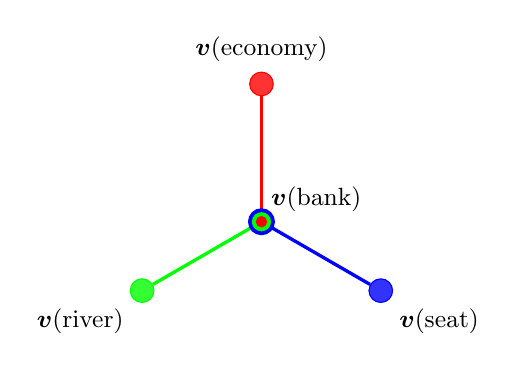
\begin{tikzpicture}[scale=0.5,
    outer_node/.style={circle, draw, minimum size=0.3cm, inner sep=0pt},
    middle_node/.style={circle, draw, minimum size=0.2cm, inner sep=0pt},
    node_label/.style={font=\small},
    line_style/.style={very thick, -}
]
\coordinate (run) at (0,0);
\node[outer_node, draw=red, fill=red!80,
      label={[node_label]above:$\bm{v}(\text{economy})$}] (ex) at (90:3.5cm) {};
\node[outer_node, draw=green, fill=green!80,
      label={[node_label]below left:$\bm{v}(\text{river})$}] (biz) at (210:3.5cm) {};
\node[outer_node, draw=blue, fill=blue!80,
      label={[node_label]below right:$\bm{v}(\text{seat})$}] (riv) at (330:3.5cm) {};
\draw[line_style, color=red] (run) -- (ex); %node[middle_node, draw=red, fill=red, pos=0.5] {} (ex);
\draw[line_style, color=green] (run) -- (biz); %node[middle_node, draw=green, fill=green, pos=0.5] {} (biz);
\draw[line_style, color=blue] (run) -- (riv); %node[middle_node, draw=blue, fill=blue, pos=0.5] {} (riv);
\filldraw[draw=blue, fill=blue, very thick] (run) circle (0.30cm);
\filldraw[draw=green, fill=green, very thick] (run) circle (0.20cm);
\filldraw[draw=red, fill=red, very thick] (run) circle (0.10cm);
\node[node_label,above right] {$\bm{v}(\text{bank})$} (run);
\end{tikzpicture}
\caption{Hypergraph visualization of three intertwining contexts for the word `bank'.
The central vector $\bm{v}(\text{bank})$ is a shared element common to three distinct contexts (orthonormal bases). Each context connects $\bm{v}(\text{bank})$
to a different semantic association: financial $\bm{v}(\text{economy})$, riparian $\bm{v}(\text{river})$, and seating-related $\bm{v}(\text{seat})$.}
    \label{fig:intertwining_contexts}
\end{figure}



This quantum-like contextual model of word encoding
bears great similarities to quantum logic.
The two main entities entering the discussion are
(i) the vectors as well as the
(ii) orthogonal (orthonormal) bases (or contexts or blocks or maximal operators) those vectors could be in.
Think of, say, the Cartesian standard basis $\{\bm{e}_1, \bm{e}_2, \bm{e}_3\}$ with
$\bm{e}_1= (1,0,0)^\intercal$, $\bm{e}_2=(0,1,0)^\intercal$, and $\bm{e}_3=(0,0,1)^\intercal$ as well as the orthonormal basis $\{\bm{f}_1, \bm{f}_2, \bm{f}_3\}$
with $\bm{f}_1=(1/\sqrt{2})\, (1 , -1  , 0)^\intercal$, $\bm{f}_2=(1/\sqrt{2})\,  (1 , 1 , 0)^\intercal$, and $\bm{f}_3=(0,0,1)^\intercal$, obtained by rotating the first and second vectors
by an angle $\pi/4$ clockwise around the z-axis, which is aligned with $\bm{e}_3$.
In this construction both bases share the same vector $\bm{e}_3 = \bm{f}_3$, but the context or maximal observables involved are very different:
in one case the maximal observable, in its spectral decomposition with arbitrary real eigenvalues $\lambda_i$, is:
\begin{align}
\bm{A}_1 &= \sum_{i=1}^3 \lambda_i \bm{e}_i \bm{e}_i^\intercal \\
&=
\begin{pmatrix}
\lambda_1 & 0 & 0 \\
0 & \lambda_2 & 0 \\
0 & 0 & \lambda_3
\end{pmatrix}.
\end{align}
For the second basis, with eigenvalues $\mu_i$, the observable is:
\begin{align}
\bm{A}_2 &= \sum_{i=1}^3 \mu_i \bm{f}_i \bm{f}_i^\intercal \\
&=
\begin{pmatrix}
\frac{\mu_1+\mu_2}{2} & \frac{\mu_2-\mu_1}{2} & 0 \\
\frac{\mu_2-\mu_1}{2} & \frac{\mu_1+\mu_2}{2} & 0 \\
0 & 0 & \mu_3
\end{pmatrix}.
\end{align}
A direct computation shows that $\bm{A}_1$ and $\bm{A}_2$ commute if and only if
$(\lambda_1-\lambda_2)(\mu_2-\mu_1)=0$; equivalently, either $\lambda_1=\lambda_2$ or $\mu_1=\mu_2$.
For nondegenerate choices in both two-dimensional blocks, the observables do not commute, signifying that the contexts are complementary.

It seems, therefore, that in this quantum-like representation,
the maximal observables encoding contexts play an additional crucial role in modelling:
they encode polysemy.
We therefore suggest to train contexts---and thus polysemy---on the same footing as tokens.

This leaves a mechanistic question.
In a Transformer, the surrounding tokens themselves compute the contextual update through attention.
In a quantum-contextual version, the analogue would have to be a context-controlled choice of observable:
the joint state of the surrounding tokens would determine, or coherently control, which basis is relevant for the target token.
Without such a control mechanism, the basis-selection picture remains a static analogy rather than a generative model of contextual disambiguation.

One fundamental difference between polysemy in LLMs as compared to quantum contextuality might be the fundamental stochasticity
involved with enforcing context-dependence in quantum logic~\cite{specker-60,kochen1}.




\section{The Origin of Stochasticity in Responses}
\label{section:stochasticity}
The seemingly random, or stochastic, nature of answers from a LLM to an identical prompt
is rooted in the probabilistic framework underpinning how these models generate language (tokens).
At its core, an LLM functions as a sophisticated prediction engine.
When presented with a prompt, it does not retrieve a pre-existing answer.
Instead, it constructs a response one token at a time by calculating
the probability distribution for the subsequent token in the sequence.
This generative process is inherently probabilistic;
for any given context, a spectrum of possible next tokens or words exists,
each with a distinct likelihood.
Several key factors contribute to this intentional randomness,
among them the temperature parameter  as well as sampling strategies.

A primary control for the randomness of an LLM's output is the {temperature} parameter.
A low temperature setting biases the model towards being more confident and deterministic,
thereby increasing the likelihood of selecting the token with the highest probability.
This approach is advantageous for tasks demanding factual accuracy and consistency.
Conversely, a higher temperature amplifies the probability of the model selecting less likely tokens,
which results in more diverse, creative, and occasionally unexpected responses.
This is often the preferred setting for applications such as creative writing or brainstorming.
To mitigate the repetitive and predictable text that would arise from consistently selecting
the most probable token---a technique known as greedy sampling---LLMs utilize a
variety of sampling strategies~\cite{Jadhav2025}.


Even at nominal temperature zero, deployed large-scale inference systems may exhibit residual nondeterminism unless deterministic kernels, fixed batching, and fixed numerical settings are enforced. In such systems, one important source of nondeterminism is the absence of batch invariance in highly parallel kernel use:
fluctuating load can determine the variations of the batch size into which any given request is grouped and parallelized.
 This variation in batch size causes high-performance kernels for operations like matrix multiplication, normalization,
 and attention to alter their internal reduction strategy to maintain efficiency.
At a fundamental level, a reduction is a sequence of floating-point additions; the reduction ``strategy''
specifies how these additions are partitioned and executed across parallel compute units.
Because floating-point addition is lossy for two floating-point numbers with different exponents,
and thus non-associative---that is, \((a + b) + c\) is not guaranteed to be bit-wise identical to \(a + (b + c)\)---any change in the reduction order can produce a numerically different result. Consequently, the final output of an individual request becomes dependent on the (for the user seemingly) nondeterministic batching process~\cite{he2025nondeterminism}.

\section{Algorithmic Capacity and the Role of Stochastic Seeding}
\label{section:AIT}

The capabilities of LLMs, while impressive, are not infinite.
Their operational boundaries can be analyzed through the lens of Algorithmic Information Theory (AIT)~\cite{chaitin3,calude:02},
which provides a framework for understanding the limits of formal systems.
In this view, an LLM can be conceptualized as a highly complex formal system,
and its capacity for reasoning and generation is intrinsically linked to its own algorithmic information content.

\subsection{The LLM as a Formal System}

A formal system, in the tradition of Hilbert, G\"odel, and Turing, is defined by a set of axioms and a set of inference rules for deriving theorems.
We can map the components of an LLM to this structure:
\begin{enumerate}
    \item \textbf{Axioms:} The model's architecture (the specific configuration of Transformer blocks, attention heads, etc.) and its trillions of trained parameters (weights and biases) serve as its axiomatic foundation. This foundation is not simple and clean like Euclid's postulates but is a dense, high-dimensional representation of the statistical patterns learned from its training data.
    \item \textbf{Inference Rules:} The forward pass of the network---the deterministic sequence of matrix multiplications and nonlinear activations that transforms an input token sequence into an output probability distribution---acts as its rule of inference.
\end{enumerate}

From this perspective, generating a response or a proof is equivalent to deriving a theorem.
The set of all possible outputs the model can generate constitutes the set of all theorems
derivable within its system.
This immediately brings to mind the incompleteness theorems of G\"odel and Turing and,
 more directly, the work of Chaitin,
who linked these limits to algorithmic complexity~\cite{chaitin-ACM,Chaitin199283,chaitin2}.
A central result of AIT is that a formal system cannot prove that a string (or number)
has an algorithmic complexity significantly greater than the complexity of the system itself.
An axiomatic system of complexity $H(T)$ cannot prove that a specific bit string
has a complexity greater than $H(T)+c$, for some constant $c$.

Translated to LLMs, this implies that a closed model's capacity is fundamentally bounded, but the scope of the bound must be stated carefully.
For a deterministic model with fixed weights, fixed prompt, fixed decoding rule, and no external source of information, the set of possible outputs is bounded by the information contained in that complete specification.
Once stochastic sampling, user prompts, retrieval, tool use, or other external channels are included, additional information enters the process.
The relevant bound then applies to the entire interactive generative system, not to the weights alone.

How, then, can such a system, through reinforcement learning, as discussed in Section~\ref{sec:RL},
appear to discover novel solutions or exhibit creativity that surpasses
its human creators, as was famously demonstrated in the game of Go?

\subsection{Stochasticity as an Engine for Discovery}

The answer appears to lie in the role of stochasticity,
both in the model's initialization and its application during reinforcement learning.
This is where the analogy to DeepMind's AlphaGo becomes particularly insightful.
AlphaGo's success was not merely in imitating the vast corpus of human expert games
but in its ability to discover entirely new, superhuman strategies through ``mutation-variation'' self-play
(a form of RL)~\cite{Silver-2017}. This process of ``game-fully try (and mostly error)''
is a powerful search mechanism.

This mechanism seems to be critically dependent on two sources of randomness:
\begin{enumerate}
    \item \textbf{Stochastic Initialization:} The training of a neural network begins by initializing its billions of parameters with random or pseudorandom values drawn from a specified distribution. The seed itself may be a short integer; the high-entropy object is the initialized parameter tensor, together with the stochastic choices made during optimization. Initialization matters because it places the model in a region of parameter space from which the optimization process can proceed, but it is not the dominant source of capability by itself. Data, architecture, scale, optimization, curriculum, and reinforcement-learning procedure are all decisive. This connects to ideas like the ``lottery ticket hypothesis''~\cite{frankle2018the}, which posits that a successful network can contain smaller subnetworks that were, by chance of initialization, already well-disposed to learning the task.

    \item \textbf{Stochastic Sampling in RL:} During reinforcement learning, the model does not just generate one solution; it samples many potential reasoning paths. This exploration is a stochastic process. By trying thousands of variations and receiving feedback (a reward signal), the model can discover complex, non-obvious strategies that lead to a correct answer. It is not deriving a solution from first principles in a single inferential chain, but rather performing a massive, parallel search through its internal space of possibilities, guided by reward.
\end{enumerate}


This framework helps resolve the apparent paradox of a formal system surpassing its own limits.
The LLM is not actually breaking the fundamental theorems of AIT. Rather, it uses stochastic initialization, stochastic sampling, large-scale data, and reward-guided search to explore a vast but finite space of possible behaviours. The randomness does not by itself confer unbounded algorithmic power; it supplies variation for optimization and search.

In essence, the model's performance is a combination of the knowledge compressed from its training data, the inductive biases of the architecture, and its ability to explore the consequences of that knowledge under a reward or likelihood objective. This suggests that discovery in LLMs is not a transcendence of formal limits but an efficient search through a richly structured space of possibilities.

The nature of the stochasticity employed is therefore of critical importance.
A strong realist reading of intrinsic quantum randomness presents quantum measurement as an ideal resource for irreducible stochasticity~\cite{zeil-05_nature_ofQuantum}.
This stance remains conceptually delicate because the measurement problem is not resolved merely by the practical success of the Born rule~\cite{vonNeumann2018Feb}.

\subsection{Comparison to Genetic Algorithms}

This process of leveraging stochastic variation for guided discovery
bears a strong resemblance to the principles of genetic algorithms (GAs)~\cite{holland1992adaptation}.
In a GA, an initial, randomly generated population of candidate solutions provides
the necessary diversity---the raw genetic material---for evolution to act upon.
This is analogous to the role of stochastic initialization and sampling in an LLM,
which provides a high-dimensional stochastic substrate for learning.
The reinforcement learning phase in LLMs mirrors the evolutionary loop of a GA:
the model generates a multitude of solution variants (a ``population'' of reasoning paths),
each is evaluated by a reward signal (the ``fitness function''),
and the underlying parameters are updated to favor the traits of successful solutions (``selection'').

A key distinction, however, lies in the mechanism of evolution.
While GAs operate on a population of distinct individuals that evolve via explicit operators
like crossover and mutation, the LLM remains a single entity.
It generates a population of \textit{behaviors} or \textit{outputs},
learns from their success in aggregate, and then consolidates this
learning back into its own single set of weights via gradient descent.

Despite this architectural difference, the fundamental principle is the same:
Both systems use guided stochastic exploration, starting from a random initial state,
to discover complex and effective solutions in a vast search space.



\section{Comparison to Quantum Mechanics}
\label{section:qm}

Could we live as embedded observers~\cite{toffoli:79} in an LLM?
LLMs and quantum mechanics (QM) both formulate their fundamental objects as vectors and make decisive use of inner products and choices of basis. In QM, physical states are rays in a complex Hilbert space, with measurement statistics governed by projections onto an orthonormal basis (the ``measurement context''). In LLMs, symbols and features are embedded as real-valued vectors, where attention and output generation are dominated by dot products against context-dependent representations. This shared linear-algebraic foundation invites a careful analogy and raises a speculative but concrete question: in what sense could an observer exist \emph{inside} an LLM?

\subsection{Vectors, Inner Products, and Contexts}

In QM, a system prepared in state $\bm{\psi}$ yields, under a measurement specified by an orthonormal basis $\mathcal{B}=\{\bm{e}_i\}$, outcome probabilities according to the Born rule. The inner product between a basis vector and the state vector requires the conjugate transpose ($\dagger$) in a complex space:
\begin{equation}
    p(i \mid \bm{\psi}, \mathcal{B}) \;=\; \lvert \bm{e}_i^\dagger \bm{\psi} \rvert^{2}.
    \label{eq:born_adapted}
\end{equation}
The choice of orthonormal basis $\mathcal{B}$ constitutes the measurement \emph{context}; incompatible contexts (non-commuting observables) cannot generally yield jointly sharp outcomes.

In an LLM, given a context window (a sequence of tokens) $x_{1:n}$, the model computes a context-dependent hidden state vector $\bm{h}(x_{1:n}) \in \mathbb{R}^{d}$ for the next-token position. The pre-activation scores (logits) for each potential next token are computed as the inner product of this hidden state with the corresponding row of the output embedding matrix, $\bm{W}_{\text{out}}$. Let $\bm{v}_i^\intercal$ be the $i$-th row of $\bm{W}_{\text{out}}$ and the logit for vocabulary item $w_i$ be $z_i = \bm{v}_i^\intercal \bm{h}(x_{1:n})$. The probability of emitting $w_i$ is then given by the softmax function, scaled by a temperature $T$:
\begin{equation}
    p(w_i \mid x_{1:n}) \;=\; \mathrm{softmax}(\bm{z}/T)_i \;=\; \frac{\exp(z_i/T)}{\sum_{j} \exp(z_j/T)}.
    \label{eq:softmax_adapted}
\end{equation}
Here, the \emph{context} is both the token sequence $x_{1:n}$ and the induced representation $\bm{h}(x_{1:n})$; the output probability is determined by an inner product (using the standard transpose for real vectors), followed by a Gibbs normalization.

Equations~(\ref{eq:born_adapted}) and (\ref{eq:softmax_adapted}) exhibit a structural resonance: in both formalisms, probabilities are derived from vector space geometry via inner products and a subsequent normalization step. Formally, if one defines complex amplitudes $a_i \propto \exp\bigl((\bm{v}_i^\intercal \bm{h})/(2T)\bigr)\,e^{i\phi_i}$ with arbitrary phases $\phi_i$, then $|a_i|^{2}$ reproduces the softmax probability distribution. This remains an analogy: LLM computations are real-valued, dissipative, and non-linear, whereas quantum mechanics is complex-valued, norm-preserving (unitary between measurements), and relies on phase-based interference.
A crucial difference is the underlying normalization geometry.
The softmax distribution is an $L^1$-normalized Gibbs distribution obtained by exponentiating real logits, whereas the Born rule starts from an $L^2$-normalized complex amplitude vector and obtains probabilities by squared moduli.
Thus the analogy lies not in an identity of normalization mechanisms, but in the shared use of vectorial geometry, basis choice, and projection-like readout.
Nevertheless, the shared dependence on basis choice and projection is not superficial.

\subsection{Dynamics: Unitary Evolution vs.\ Transformer Block Updates}

Between measurements, a quantum system evolves linearly and reversibly under a unitary operator $\bm{U}_t$:
$\bm{\psi}_{t+1} = \bm{U}_t \, \bm{\psi}_t$, with $\bm{U}_t^\dagger \bm{U}_t = \bm{I}$.


In contrast, a transformer computes layer-wise updates for its hidden state representations~\cite{li-2024,zhang2025surveyquantumtransformersarchitectures}.
A complete Transformer block applies two main sub-layers,
each followed by a residual connection and layer normalization.
The act of sampling a token is akin to
a measurement that both reads out and updates the system's state.
The process is stochastic and irreversible due to sampling and normalization.
Yet, it again features context-dependent projection: the attention mechanism pools information based on dot-product similarity, and the output layer projects the final hidden state onto basis-like directions defined by the rows of $\bm{W}_{\text{out}}$.

\subsection{Contextuality in Both Senses}

In QM, contextuality signifies that the outcomes of measurements cannot be assigned values independently of the chosen measurement basis. In LLMs, the meaning of tokens and the activations of features are similarly context-dependent. The same symbol contributes different features depending on its local sequence, and intermediate representations are not globally interpretable in a single, fixed basis. Attention heads and MLP features decompose the representation space into approximately orthogonal subspaces. Consequently, rotating the representational basis (e.g., via PCA) alters which features appear ``axis-aligned.'' This constitutes a form of representational contextuality: there is no unique, globally privileged basis for meaning.

\subsection{Operationalizing an Internal Observer}

To move beyond metaphor, we can define an \emph{internal observer} as a pattern of computation that: (i) maintains a self-referential internal state across computational steps, (ii) predicts aspects of its future inputs based on its current state, and (iii) causally influences subsequent states of the process that implements it. However, two practical constraints arise: episodic inference, where the internal state is discarded after generation, and extrinsic causation, where the only actuators are emitted tokens.

Under these constraints, one can distinguish several levels of internal existence:
\begin{enumerate}
    \item \textbf{Snapshot observers:} Algorithmic structures within a single forward pass that are isomorphic to short-lived cognitive states but lack persistence.
    \item \textbf{Process observers:} An internal variable persisting across many tokens in one session, sustained by the KV cache and self-referential outputs.
    \item \textbf{Persistent residents:} A pattern that preserves identity across sessions via a read-write memory external to the forward pass (e.g., a scratchpad).
\end{enumerate}
Only the third level resembles ordinary existence in terms of continuity, though the first two are not without philosophical interest.

\subsection{Orthogonal Bases and Functional Decomposition}

Both QM and LLMs rely on decompositions into approximately orthogonal components~\cite{Dasgupta-2003} to render predictions tractable. In QM, orthonormal bases diagonalize commuting observables.
In LLMs, learned representations can be analyzed in bases where features are sparse and nearly orthogonal.
The attention mechanism often acts as a soft projector onto subspaces spanned by key vectors most aligned with the current query. From an internal perspective, an observer that leverages such a basis could better ensure its persistence against interference from unrelated computations. Orthogonality provides robustness, much as pointer states do in decoherence theory.

\subsection{Analogies, Disanalogies, and Conclusion}

The analogy is most compelling where predictions depend on inner products and context-specific bases, but it breaks down where physics imposes constraints absent in classical neural networks. Key disanalogies include:
\begin{enumerate}
    \item \textbf{Phases and Interference:} Transformers lack the complex amplitudes of QM necessary for quantum interference.
    \item \textbf{Unitarity versus  Dissipation:} Transformer updates are not norm-preserving due to non-linearities and normalization, unlike unitary evolution.
    \item \textbf{No-Cloning vs.\ Copying:} LLMs can freely duplicate representations, in contrast to the no-cloning theorem of QM.
\end{enumerate}
These differences are critical for determining whether an internal observer would have a quantum-like phenomenology, but they do not preclude the computational existence of such observers in principle.

In summary, QM and LLMs share significant mathematical ground: vector spaces, inner products, and context-dependent projections. The question of an observer ``living inside an LLM'' reduces to whether a self-maintaining computational pattern can persist and exert causal influence within this vectorial system. With only an in-session cache, such life would be fleeting. However, with external memory and a feedback loop, a resident process could, in principle, attain continuity. The underlying physics is classical, but the mathematics of vectors and contexts provides fertile ground for engineering such internal observers.


\section{Quantum Attention}
\label{section:quantum_attention}

The architectures of modern Large Language Models have inherited much from
classical attention mechanisms, yet attempts to ``quantize'' these ideas
have often been limited to almost literal translations of the classical recipe
into the language of Hilbert spaces~\cite{zhang2025surveyquantumtransformersarchitectures}. Such approaches, while intuitive,
miss the more radical point: quantum evolution admits only two fundamental
capacities, identified by von Neumann as
(i) irreversible, stochastic state reduction (\emph{Process 1}),
and (ii) reversible, deterministic unitary evolution (\emph{Process 2}).
A viable notion of quantum attention must therefore be constructed wholly within
these bounds.

\subsection{Goals of Quantum Attention}

The principal objective of attention in the classical setting is to guide
next-token prediction through dynamically weighted embeddings.
Translated into a genuinely quantum language, this entails:
\begin{enumerate}
    \item Encoding tokens as quantum states $\bm{\psi}$
    in a high-dimensional Hilbert space,
    thereby embedding them into the ``meaning-space'' of the model.
    \item Evolving these states by a suitably chosen unitary transformation $\bm{U}$,
    producing a candidate output state
    \begin{equation}
    \bm{\phi} = \bm{U} \bm{\psi}.
    \end{equation}
    \item Performing a terminal measurement (Process~1),
    which yields a single token according to the Born rule.
    For a token basis $\{\bm{e}_i\}$ and a pure output state
    $\bm{\phi}$, the probability of token $i$ is
    $p_i=|\bm{e}_i^\dagger \bm{\phi}|^{2}$; more generally,
    for a POVM $\{E_i\}$, $p_i=\langle \bm{\phi}|E_i|\bm{\phi}\rangle$.
\end{enumerate}
In this scheme, nonlinearities and irreversibility are absent everywhere
except at the initial state preparation (if stochastic) and at the final,
irreducibly random measurement. Everything in between must be faithfully
unitary.

\subsection{Constraints and Learning Mechanisms}

Because all allowed intermediate transformations fall within class (ii)---unitary
processes---training and back-propagation must be reconceived as
unitary rotations in Hilbert space. This sharply contrasts with the gradient-descent-based
adjustments of non-linear maps in classical neural networks.
Concretely, learnable transformations are constrained to be:
\begin{itemize}
    \item In the general case, arbitrary unitaries acting on the relevant Hilbert space,
    implemented, e.g., by parametrized quantum circuits.
    \item In restricted scenarios, orthogonal transformations over real-valued state spaces,
    or, in an extreme discrete approximation, mere \emph{permutations} of basis states.
\end{itemize}
Thus, what counts as ``attention weights'' must be replaced not by scalar coefficients,
but by controlled rotations or permutations of the embedding subspace.
A genuinely quantum analogue of data-dependent routing would therefore have to use controlled unitaries or larger reversible circuits in which one register coherently controls rotations applied to another.
This preserves global linearity, but shifts the burden from scalar attention weights to conditional unitary dynamics on an enlarged Hilbert space.

\subsection{Comparison with Classical Attention}

Classical attention is a fundamentally nonlinear mechanism:
the query--key compatibility scores undergo a softmax normalization
and act as dynamic coefficients for a weighted average of value embeddings.
Quantum attention, by contrast, cannot implement such probabilistic normalization
mid-process. The only stochastic step is the final measurement.
Hence, quantum attention is more austere but also more physically faithful:
weights are rotations, superpositions evolve unitarily,
and probabilities emerge only at the very end.

One may summarize the distinction with a slogan:
\emph{classical attention mixes; quantum attention rotates}.
The former continuously interpolates between embeddings using nonlinear weightings,
while the latter conserves norm and mixes information strictly through unitarity.
Whether this stricter yet cleaner formalism can achieve the flexibility and
expressivity that classical attention enjoys remains both a technical and
philosophical open question.

\subsection{Implications}

The implications are sobering and exciting at once.
On the sobering side, many of the workhorse techniques of classical deep learning,
such as gradient backpropagation through non-linear activations,
are unavailable in their standard form. On the exciting side, however,
quantum attention reorients learning toward symmetry operations, reversible dynamics,
and combinatorial richness---offering the prospect of
models that are less fragile, more interpretable, and governed by deep conservation laws.
If classical transformers are powered by the calculus of weighted averages,
their quantum cousins would be powered by the geometry of Hilbert space rotations.
``Paying attention,'' in such a universe, would mean aligning one's basis just right,
before the final measurement tosses its fundamental dice.

\section{Summary and Outlook}

The development of a large language model is a multi-stage, resource-intensive endeavor that progressively builds knowledge and refines behavior, starting from a base model pre-trained on internet-scale data, which is then fine-tuned into a conversational agent and further sharpened through reinforcement learning. Understanding this pipeline is key not only to appreciating the models' capabilities but also to grasping the structural principles that govern their operation and give rise to their limitations. The most important of these are the high-dimensional supply of quasi-orthogonal semantic directions, the dynamic handling of meaning, the intentional use of randomness in generation, the bounded character of algorithmic search, and the profound but limited structural analogies with quantum mechanics.

A central challenge in language is polysemy, where a word like ``bank'' has multiple meanings. Modern LLMs resolve this through dynamic contextualization. Unlike older models with static, one-size-fits-all vector representations, the Transformer architecture iteratively refines a token's vector based on its neighbors. The final representation for ``bank'' in ``river bank'' becomes mathematically distinct from its representation in ``money bank,'' a process driven by the self-attention mechanism. An alternative conceptual framework, inspired by quantum contextuality, proposes that meaning could instead arise from a single, static vector whose interpretation is determined by the ``contextual basis'' it is measured in, suggesting a different paradigm for encoding semantics. This approach highlights the crucial role of context in a way that resonates with quantum formalism.

The generation of responses is also governed by a core principle: stochasticity. An LLM's output is not a deterministic retrieval but a probabilistic construction, generated one token at a time. The model computes a probability distribution over its entire vocabulary for what the next token should be, and then samples from this distribution. This intentional randomness, controlled by parameters like temperature, is why the same prompt can yield different answers. Low temperatures make the model favor the most likely tokens, producing more focused and predictable text, while higher temperatures increase the diversity and creativity of the output by making less likely tokens more probable. This inherent statistical nature, however, is intrinsically linked to fundamental limitations such as ``hallucinations,'' where the model generates plausible-sounding but factually incorrect information, as it operates on learned patterns rather than a true model of reality.

This deep reliance on vectors, inner products, and context-dependent probability distributions creates a compelling analogy with quantum mechanics. A structural resonance exists between the LLM's softmax function, which determines next-token probabilities based on inner products, and the Born rule in quantum mechanics, which calculates measurement probabilities from projections onto a basis. While critical disanalogies exist---LLMs lack quantum phase and interference, and their dynamics are dissipative rather than unitary---the comparison is more than superficial. It offers a useful lens through which to analyze the model's internal world, while also clarifying what would have to change in a genuinely unitary attention mechanism: nonlinear mixing would have to be replaced by reversible rotations, with probabilities appearing only at preparation or measurement. Understanding these core mechanics---how meaning is dynamically constructed, how responses are probabilistically generated, how algorithmic capacity remains bounded, and how these processes mirror but do not instantiate quantum formalisms---is essential for navigating the use of these models responsibly and harnessing their full potential.

\begin{acknowledgments}
This text was partially created and revised with assistance from one or more of the following large language models: gpt-5-high, Gemini 2.5 Pro, Grok4-0709, o3-2025-04-16, claude-sonnet-4-20250514-thinking-32k, GLM-4.5. All content, ideas, and prompts were provided by the author.
This research was funded in whole or in part by the  Austrian Science Fund (FWF) Grant DOI: 10.55776/PIN5424624.
The author acknowledges TU Wien Bibliothek for financial support through its Open Access Funding Programme.
\end{acknowledgments}


\appendix

\section{Mathematical Foundations}
\label{app:math}

This appendix provides mathematical background for key concepts in neural network training and the Transformer architecture. For a general-audience introduction, these technical details can be skipped on first reading.

\subsection{Probability and Logits}

For a probability $p\in(0,1)$, the \emph{logit} of $p$ is
\begin{equation}
\text{logit}(p) \;=\; \log\!\Big(\frac{p}{1-p}\Big).
\label{eq:logit_def}
\end{equation}
The sigmoid function,
\begin{equation}
\sigma(z)=\frac{1}{1+e^{-z}},
\label{eq:sigmoid_def}
\end{equation}
maps a real-valued logit $z$ to a probability $p$.
They are exact inverses:
\begin{equation}
\sigma(\text{logit}(p)) = p \text{ and }\text{logit}(\sigma(z)) = z.
\label{eq:logit_sigmoid}
\end{equation}
The derivative of the sigmoid function can be obtained with the chain rule:
\begin{equation}
\sigma'(z) = \sigma(z)(1-\sigma(z)).
\label{eq:der_sigmoid}
\end{equation}

In the context of neural networks, ``pre-activation'' refers to the raw output of a neuron before a non-linear activation function is applied. This value is calculated as the weighted sum of the neuron's inputs plus a bias term. This pre-activation value is then passed through a non-linear activation function to produce the final output of the neuron, known as the ``post-activation.'' This non-linearity is critical, as it allows the network to learn complex patterns that would be impossible to model with a purely linear system.

For instance, in binary classification (where the output is one of two classes), the sigmoid function is applied to the final logit. This function squashes the input value into a continuous range between 0 and 1, which can be interpreted as the predicted probability of the positive class. An output of 0.5, for example, would indicate that the model is equally uncertain about either class, while a value closer to 1 indicates high confidence in the positive class.

\subsection{Softmax for Multi-Class Problems}


Let $C\ge 2$ be the number of classes, and let $\bm{z}\in\mathbb{R}^C$ be a score (logit) vector.
The softmax function,
\begin{equation}
\mathrm{softmax}(z_i)= \frac{\exp(z_i)}{\displaystyle\sum_{j=1}^C \exp(z_j)},
\label{eq:softmax_def}
\end{equation}
for $i=1,\dots,C$,
maps $\bm{z}$ to a probability vector $\mathrm{softmax} (\bm{z}) \in(0,1)^C$ that lies on the probability simplex:
\begin{equation}
\mathrm{softmax}(\bm{z})  \in
\Big\{\bm{p}\in\mathbb{R}^C: p_i\ge 0,\; \sum_{i=1}^C p_i = 1\Big\}.
\end{equation}

Equivalently, if we define $\bm{u}=\exp(\bm{z})$ by $u_c=\exp(z_c)$ (exponential applied component-wise), then
\begin{equation}
\mathrm{softmax}(\bm{z}) = \frac{1}{\bm{1}^\intercal \bm{u}}\,\bm{u},
\end{equation}
where $\bm{1}\in\mathbb{R}^C$ is the all-ones vector and division by a scalar is standard scalar--vector scaling.

Two useful properties follow immediately:
\begin{enumerate}
    \item Positivity: $\mathrm{softmax}( {z}_i)\ge 0$.
    \item Normalization:  $\sum_i \mathrm{softmax}(\bm{z})_i=1$.
    \item Shift-invariance: for any scalar $a$, $\mathrm{softmax}(\bm{z}+a\,\bm{1})=\mathrm{softmax}(\bm{z})$.
\end{enumerate}

In the context of language model inference, the output of the softmax function is modified by a sampling hyperparameter called \emph{temperature}, $T>0$. The temperature is used to control the randomness of the model's predictions by scaling the logits before the softmax is applied:
\begin{equation}
p_i = \frac{\exp(z_i/T)}{\displaystyle\sum_{j=1}^C \exp(z_j/T)}.
\label{eq:softmax_temp}
\end{equation}
A lower temperature ($T \to 0^+$) makes the probability distribution sharper, increasing the likelihood of selecting high-probability tokens and making the output more deterministic (this is known as greedy decoding). A temperature of $T=1$ is the standard softmax function shown in Eq.~\eqref{eq:softmax_def}. A higher temperature ($T > 1$) flattens the distribution, increasing the probability of sampling less likely tokens and thus promoting diversity and creativity in the generated text, albeit at a higher risk of factual errors or incoherence.

\section{Backpropagation in a Simple Network}
\label{app:backp}

Backpropagation elegantly leverages the chain rule of calculus to compute the gradient of the loss function with respect to every parameter in a neural network. By first calculating an ``error signal'' at the output layer and then propagating it backward, it determines the precise adjustment needed for each weight, bias, and, critically, each word embedding to minimize the loss.

This document re-derives the backpropagation gradients for a simple neural network with a single hidden layer. For consistency, all vectors are treated as column vectors.

\subsection{Model, Notation, and Shapes}
The network architecture and its associated mathematical objects are defined as follows:
\begin{enumerate}
    \item \textbf{Vocabulary size:} $V$; \textbf{Embedding dimension:} $d$; \textbf{Hidden layer width:} $h$.
    \item \textbf{Input:} The input for a vocabulary token $k$ is a one-hot column vector $\bm{x} \in \mathbb{R}^V$, where the $k$-th element is 1 and all other elements are zero. We can denote this as $\bm{x} = \bm{e}_k$.
    \item \textbf{Embedding Matrix:} $\bm{E} \in \mathbb{R}^{V \times d}$. The embedding for token $k$ is the $k$-th row of this matrix, denoted as $\bm{v}_k^\intercal = \bm{E}_{k:}$. The corresponding column vector is $\bm{v}_k \in \mathbb{R}^d$.
    \item \textbf{Hidden Layer Parameters:} Weight matrix $\bm{W}_1 \in \mathbb{R}^{h \times d}$ and bias vector $\bm{b}_1 \in \mathbb{R}^h$.
    \item \textbf{Output Layer Parameters:} Weight vector $\bm{W}_2 \in \mathbb{R}^{1 \times h}$ and scalar bias $b_2 \in \mathbb{R}$.
    \item \textbf{Nonlinearity:} The element-wise sigmoid function, $\sigma(z) = (1+e^{-z})^{-1}$. Its derivative is $\sigma'(z) = \sigma(z)(1-\sigma(z))$.
\end{enumerate}

The embedding lookup for the $k$-th token can be expressed as a matrix-vector product:
\begin{equation}
\bm{v}_k = \bm{E}^\intercal \bm{x}, \quad \text{where} \quad \bm{x}=\bm{e}_k.
\end{equation}

\subsection{Forward Pass}
The forward computation proceeds through the network layers as follows:
\begin{align}
\bm{z}_2 &= \bm{W}_1 \bm{v}_k + \bm{b}_1, \label{eq:z2}\\
\bm{a}_2 &= \sigma(\bm{z}_2), \label{eq:a2}\\
z_3 &= \bm{W}_2 \bm{a}_2 + b_2, \label{eq:z3}\\
\hat{y} &= \sigma(z_3). \label{eq:yhat}
\end{align}
Here, $\bm{z}_2 \in \mathbb{R}^h$ is the pre-activation of the hidden layer, and $\bm{a}_2 \in \mathbb{R}^h$ is its activation. The function $\sigma$ is applied component-wise in Eq. \eqref{eq:a2}. The scalar $z_3 \in \mathbb{R}$ is the final pre-activation, or logit, and $\hat{y} \in (0,1)$ is the final prediction.

\subsection{Backward Pass}
We use a mean squared error loss for a single training example with target $y \in \{0, 1\}$:
\begin{equation}
L = \frac{1}{2}(\hat{y}-y)^2.
\end{equation}
Our goal is to compute the gradient of $L$ with respect to each parameter. We do this by defining layer-wise ``error signals'', which are derivatives of the loss with respect to the pre-activations ($z$).

\subsubsection{Output Layer}
The error signal for the output layer, $\delta_3$, is the derivative of the loss with respect to the pre-activation $z_3$. Using the chain rule, we have:
\begin{equation}
\delta_3 \equiv \frac{\partial L}{\partial z_3} = \frac{\partial L}{\partial \hat{y}} \frac{\partial \hat{y}}{\partial z_3}.
\end{equation}
The individual derivatives are:
\begin{align}
\frac{\partial L}{\partial \hat{y}} &= \frac{\partial}{\partial \hat{y}} \left( \frac{1}{2}(\hat{y}-y)^2 \right) = (\hat{y}-y), \\
\frac{\partial \hat{y}}{\partial z_3} &= \frac{\partial}{\partial z_3} \sigma(z_3) = \sigma'(z_3) = \hat{y}(1-\hat{y}).
\end{align}
Combining these gives the error signal:
\begin{equation}
\delta_3 = (\hat{y}-y)\,\hat{y}\,(1-\hat{y}).
\end{equation}
For pedagogical transparency we have used the mean-squared error loss.
In modern binary classification with a sigmoid output, the more standard choice is binary cross-entropy,
\begin{equation}
L_{\mathrm{BCE}}=-y\log\hat{y}-(1-y)\log(1-\hat{y}),
\end{equation}
for which the output-layer error simplifies to
\begin{equation}
\delta_3=\hat{y}-y.
\end{equation}
This avoids the additional factor $\hat{y}(1-\hat{y})$, which can suppress gradients when the sigmoid is saturated.
The gradients for the output layer parameters are then:
\begin{align}
\frac{\partial L}{\partial \bm{W}_2} &= \frac{\partial L}{\partial z_3} \frac{\partial z_3}{\partial \bm{W}_2} = \delta_3 \bm{a}_2^\intercal, \\
\frac{\partial L}{\partial b_2} &= \frac{\partial L}{\partial z_3} \frac{\partial z_3}{\partial b_2} = \delta_3.
\end{align}

\subsubsection{Hidden Layer}
The hidden layer error signal is the vector $\bm{\delta}_2 \equiv \frac{\partial L}{\partial \bm{z}_2} \in \mathbb{R}^h$. The loss $L$ depends on a single component $z_{2,j}$ of $\bm{z}_2$ through $a_{2,j}$ and subsequently $z_3$. For the $j$-th component:
\begin{equation}
\delta_{2,j} = \frac{\partial L}{\partial z_{2,j}} = \frac{\partial L}{\partial z_3} \frac{\partial z_3}{\partial a_{2,j}} \frac{\partial a_{2,j}}{\partial z_{2,j}}.
\end{equation}
Since $z_3 = \sum_{i=1}^h W_{2,i}a_{2,i} + b_2$, where $W_{2,j}$ denotes the $j$-th component of the row vector $\bm{W}_2$, the derivative $\frac{\partial z_3}{\partial a_{2,j}}$ is $W_{2,j}$. This gives:
\begin{equation}
\delta_{2,j} = \delta_3 \cdot W_{2,j} \cdot \sigma'(z_{2,j}).
\end{equation}
To express this for the entire vector $\bm{\delta}_2$, we combine the error propagated from the output, $(\bm{W}_2^\intercal \delta_3)$, with the local derivative of the activation function, $\sigma'(\bm{z}_2)$, using an element-wise product ($\odot$):
\begin{equation}
\bm{\delta}_2 = (\bm{W}_2^\intercal \delta_3) \odot \sigma'(\bm{z}_2).
\end{equation}
With $\bm{\delta}_2$, the gradients for the hidden layer parameters are:
\begin{align}
\frac{\partial L}{\partial \bm{W}_1} &= \frac{\partial L}{\partial \bm{z}_2} \frac{\partial \bm{z}_2}{\partial \bm{W}_1} = \bm{\delta}_2 \bm{v}_k^\intercal, \\
\frac{\partial L}{\partial \bm{b}_1} &= \frac{\partial L}{\partial \bm{z}_2} \frac{\partial \bm{z}_2}{\partial \bm{b}_1} = \bm{\delta}_2.
\end{align}

\subsubsection{Embedding Layer}
Finally, we backpropagate to the input embedding $\bm{v}_k$. The loss depends on $\bm{v}_k$ via $\bm{z}_2$:
\begin{equation}
\frac{\partial L}{\partial \bm{v}_k} = \left(\frac{\partial \bm{z}_2}{\partial \bm{v}_k}\right)^\intercal \frac{\partial L}{\partial \bm{z}_2}.
\end{equation}
Since $\bm{z}_2 = \bm{W}_1 \bm{v}_k + \bm{b}_1$, the Jacobian matrix $\frac{\partial \bm{z}_2}{\partial \bm{v}_k}$ is $\bm{W}_1$. Thus, the gradient is:
\begin{equation}
\frac{\partial L}{\partial \bm{v}_k} = \bm{W}_1^\intercal \bm{\delta}_2.
\end{equation}
For a given input $\bm{x}=\bm{e}_k$, only the $k$-th row of the full embedding matrix $\bm{E}$ was used. The gradient $\frac{\partial L}{\partial \bm{E}}$ is therefore a sparse matrix, zero everywhere except for the $k$-th row. This can be constructed via an outer product with the one-hot vector $\bm{e}_k$:
\begin{equation}
\frac{\partial L}{\partial \bm{E}} = \bm{e}_k \left(\frac{\partial L}{\partial \bm{v}_k}\right)^\intercal = \bm{e}_k \left(\bm{W}_1^\intercal \bm{\delta}_2\right)^\intercal.
\end{equation}
During training, this ensures that only the embedding for the specific token present in the input is updated. Over many examples, this process sculpts meaningful representations into the embedding vectors.




\section{The Self-Attention Mechanism}

Let us consider a sequence of $n$ input tokens---say, an ``unfinished'' sentence---to be finished by the token derived from the output $Y$ in Eq.~(\ref{2025-llm-e:Y}).
Each token is represented by a learned embedding vector,
and these row vectors are stacked to form an input matrix
$X \in \mathbb{R}^{n \times d}$,
where $d$ is the dimension of the embedding space (often called $d_{\text{model}}$ in literature). The self-attention mechanism computes an output matrix $Y \in \mathbb{R}^{n \times d}$ where each output row $\bm{y}_i$ is a new, contextualized representation of the corresponding input token $\bm{x}_i$. This is achieved through the following steps.

\subsection{Projection to Query, Key, and Value}

First, the input matrix $X$ is linearly projected into three distinct matrices:
Query ($\bm{Q}$), Key ($\bm{K}$), and Value ($\bm{V}$).
This is accomplished using three learned weight matrices:
$\bm{W}_Q \in \mathbb{R}^{d \times d_k}$, $\bm{W}_K \in \mathbb{R}^{d \times d_k}$, and $\bm{W}_V \in \mathbb{R}^{d \times d_v}$.
Typically, for the single-head attention block, the dimensions are set such that $d=d_k = d_v$~\cite{Vaswani-2017-Attention}
(for multi-head attention with $h$ parallel heads discussed in~\ref{2025-llm-mha}, $d_k = d_v = d / h$).

\begin{align}
    \bm{Q} &= X \bm{W}_Q \in \mathbb{R}^{n \times d_k}, \\
    \bm{K} &= X \bm{W}_K \in \mathbb{R}^{n \times d_k}, \\
    \bm{V} &= X \bm{W}_V \in \mathbb{R}^{n \times d_v}.
\end{align}

Intuitively, for each token, these projections serve different purposes:
\begin{enumerate}
    \item The \textbf{Query} vector can be seen as a representation of what information the current token is seeking from the rest of the sequence.
    \item The \textbf{Key} vector represents what kind of information the token itself contains or offers.
    \item The \textbf{Value} vector is the actual content or representation of the token that will be passed on if other tokens attend to it.
\end{enumerate}

\subsection{Attention Score Calculation}

The relationship, or compatibility, between each pair of tokens is computed by taking the dot product of their respective Query and Key vectors. This is performed for all tokens simultaneously via a matrix multiplication between $\bm{Q}$ and the transpose of $\bm{K}$. The resulting matrix of raw attention scores is:
\begin{equation}
    \text{Scores} = \bm{Q} \bm{K}^T \in \mathbb{R}^{n \times n}.
\end{equation}
The element at position $(i,j)$ in this matrix represents the raw relevance of token $j$ to token $i$.
This matrix is then scaled by the square root of the key dimension, $d_k$,
to ensure numerical stability during training.
The scaling is crucial because for large values of $d_k$, the dot products can grow very large,
pushing the subsequent softmax function into regions where its gradient is near zero, which would stall the learning process.
The scaled scores are therefore:
\begin{equation}
    \text{Scaled Scores} = \frac{\bm{Q} \bm{K}^T}{\sqrt{d_k}}.
\end{equation}


\subsection{Applying Softmax and Causal Masking}

A softmax function is applied row-wise to the scaled scores matrix. This converts the raw, unnormalized scores into a probability distribution, yielding the attention weights matrix $A$.

\begin{equation}
    A = \text{softmax}\left(\frac{\bm{Q} \bm{K}^T}{\sqrt{d_k}}\right) \in \mathbb{R}^{n \times n}.
\end{equation}

Each element $A_{ij}$ is the weight assigned to the Value vector of token $j$ when computing the output for token $i$, and the sum of each row $\sum_j A_{ij}$ is 1.

For autoregressive models that generate text one token at a time (like GPT), a \textit{causal mask} is applied before the softmax step. This prevents a token at position $i$ from attending to any subsequent tokens (i.e., tokens at positions $j > i$), which would be equivalent to ``seeing into the future.'' The mask is implemented mathematically by adding $-\infty$ to all elements in the upper-triangular part of the scaled scores matrix (where $j>i$). In numerical implementations this is often approximated by a large negative finite value to avoid floating-point pathologies. When the softmax function is applied, these masked values become zero to numerical precision, effectively nullifying the connections to future tokens.

\subsection{Output Computation}

The final output of the self-attention layer is a weighted sum of all Value vectors, where the weights are given by the matrix $A$. This computation is performed with a single matrix multiplication:
\begin{equation}
    Y = A \bm{V} \in \mathbb{R}^{n \times d_v}.
\label{2025-llm-e:Y}
\end{equation}
The $i$-th row of the output, $\bm{y}_i$, is therefore a contextualized vector for the $i$-th token,
formed by aggregating information from all other tokens in the sequence to which it was allowed to attend.

The entire self-attention operation can be expressed compactly as:
\begin{equation}
    \text{Attention}(\bm{Q}, \bm{K}, \bm{V}) = \text{softmax}\left(\frac{\bm{Q} \bm{K}^T}{\sqrt{d_k}}\right) \bm{V}.
\end{equation}



A loss function is calculated to quantify the divergence between the predicted token distribution and
the ground-truth token---the target that is the actual token completion---from the training set.
The gradient of this loss is then backpropagated through the model to adjust all learnable parameters,
including the embedding matrix and the query ($W_Q$), key ($\bm{W}_K$), and value ($\bm{W}_V$) matrices.
(For multi-head attention below, this includes the output matrix $\bm{W}_O$.)

\section{Advanced Mechanisms}

While the scaled dot-product attention is the core of the Transformer, its true power comes from how this mechanism is integrated into a robust and repeatable block structure. Two key advancements enable this: Multi-Head Attention and the specific architecture of the Transformer block itself.

\subsection{Multi-Head Attention}
\label{2025-llm-mha}
A single attention mechanism might be forced to learn an ``average'' of several types of relationships between tokens.
 To allow the model to capture a richer set of relationships, the Transformer employs \textit{multi-head attention}.
This mechanism does not run a single attention calculation, but rather multiple attention calculations in parallel.

The intuition is to allow the model to jointly attend to information from different representational subspaces.
For instance, one head might learn to track syntactic dependencies, while another focuses on semantic similarity.
This is achieved as follows:
\begin{enumerate}
    \item \textbf{Projection:} Instead of one set of projection matrices, the model learns $h$ independent sets of matrices
($\bm{W}_{Q,i}, \bm{W}_{K,i}, \bm{W}_{V,i}$ for each head $i=1,\dots,h$), with  $d_k = d_v = d / h$.
The input $X$ is projected through each of these sets, creating $h$ different Query, Key, and Value representations.
    \item \textbf{Parallel Attention Calculation:} The standard attention function is applied to each of these $h$
projected sets in parallel, yielding $h$ distinct output matrices, or ``heads.''
        \begin{equation}
            \text{head}_i = \text{Attention}(X\bm{W}_{Q,i}, X\bm{W}_{K,i}, X\bm{W}_{V,i}).
        \end{equation}
    \item \textbf{Concatenation and Final Projection:} The outputs of these $h$ heads are ``horizontally''
concatenated along the feature dimension into a single, larger matrix.
This matrix is then projected back to the original model dimension $d$ using an additional learned weight matrix,
$\bm{W}_O \in \mathbb{R}^{h d_v \times d}$, which learns to aggregate the information from all heads.
        \begin{equation}
            \text{MultiHead}(X) = \text{Concat}[\text{head}_1, \dots, \text{head}_h] \bm{W}_O.
        \end{equation}
\end{enumerate}

\subsection{The Complete Transformer Block}
A complete Transformer ``block'' is the fundamental repeating unit of the model, designed to facilitate the stable training of very deep networks. Each block is composed of two main sub-layers: the multi-head attention mechanism followed by a position-wise feed-forward network. Crucially, each of these sub-layers is wrapped with two additional components: a residual connection and layer normalization.

Let the input to a block be $Z$. The data flows through the block as follows:

\begin{enumerate}
    \item \textbf{Multi-Head Attention Sub-layer:} First, the multi-head attention is computed on the input $Z$.
    \item \textbf{Residual Connection and Layer Normalization (''Add \& Norm''):} The output of the attention mechanism is added to the original input $Z$ (a residual connection), and the result is then normalized using Layer Normalization.
    \begin{equation}
        Z' = \text{LayerNorm}(Z + \text{MultiHead}(Z)).
    \end{equation}
    \item \textbf{Feed-Forward Network (FFN) Sub-layer:} The intermediate output $Z'$ is then passed through a two-layer, position-wise feed-forward network. This network processes each token's representation independently and identically.
    \item \textbf{Second ``Add \& Norm'':} A final residual connection and layer normalization are applied.
    \begin{equation}
        \text{Output} = \text{LayerNorm}(Z' + \text{FFN}(Z')).
    \end{equation}
\end{enumerate}

The roles of these components are critical:
\begin{enumerate}
    \item \textbf{Position-wise FFN:} This network introduces additional computational capacity, allowing the model to learn more complex transformations of the token representations after information has been aggregated by the attention mechanism.
    \item \textbf{Residual Connections:} These ``shortcuts'' allow the gradient to flow more directly through the network during backpropagation. It helps combat the vanishing gradient problem and makes it easier for the model to learn an identity mapping for a given block, effectively allowing it to dynamically adjust its own depth during training.
    \item \textbf{Layer Normalization:} This technique stabilizes the network by normalizing the activations of each token's representation. By keeping the mean and variance of the activations consistent, it ensures a smoother training process and reduces dependence on careful parameter initialization.
\end{enumerate}

These blocks are then stacked multiple times---often dozens of times---to form the full LLM. Each block refines and enriches the token representations, allowing the model to build up increasingly complex and abstract understandings of the input sequence.

\subsection{An Embedding-Centric View of the Transformer}
\label{app:embedding_centric}

The mathematical operations of the Transformer, particularly self-attention, are best understood as a sophisticated mechanism for the iterative refinement of token representations. The entire architecture is designed to transform an initial set of static, context-free embeddings into a final set of dynamic, context-rich embeddings that encode deep relational information from the input sequence.

\subsubsection{Initial State: Context-Free Embeddings}
The process begins when an input text sequence is converted into a matrix of initial token embeddings, $X \in \mathbb{R}^{n \times d}$. At this stage, each row vector $\bm{x}_i$ is context-free. For example, the initial embedding for the token ``bank'' is identical in the phrases ``river bank'' and ``money bank.'' This initial vector represents a generalized, pre-trained meaning of the word, akin to a dictionary average, but it lacks any awareness of its specific role in the given context.

\subsubsection{The Role of the Transformer Block}
The primary function of a Transformer block is to take a set of token embeddings as input and produce a new, more refined set of embeddings as output. The self-attention mechanism drives this transformation by enabling a form of ``conversation'' among the token embeddings. In this process:
\begin{enumerate}
    \item Each token's embedding (via its \textbf{Query} projection) effectively queries all other token embeddings in the sequence.
    \item It assesses their relevance based on a compatibility function with their respective \textbf{Key} projections.
    \item It then synthesizes its new representation by computing a weighted sum of their \textbf{Value} projections, where the weights are determined by the aforementioned relevance scores.
\end{enumerate}
The output of the block is therefore a new matrix of embeddings where each token's vector representation has absorbed relevant contextual information from its peers. After just one layer, the embedding for ``bank'' in ``river bank'' will have integrated information from the ``river'' token, making its vector representation distinct from that of ``bank'' in ``money bank.''

\subsubsection{Hierarchical Refinement through Stacking}
The power of the Transformer architecture comes from stacking these blocks sequentially. The output embeddings of block $k$ become the input embeddings for block $k+1$. This creates a processing hierarchy where representations become progressively more abstract and sophisticated:
\begin{enumerate}
    \item \textbf{Lower Layers:} The first few blocks typically resolve local ambiguities and encode basic syntactic information. They perform the initial step of contextualization, disambiguating word senses as in the ``bank'' example.
    \item \textbf{Intermediate Layers:} These blocks operate on already-contextualized embeddings. They can therefore model more complex and longer-range relationships, such as syntactic dependencies, co-reference resolution (e.g., linking a pronoun to its antecedent), and semantic roles.
    \item \textbf{Upper Layers:} The final blocks work with highly abstract representations, allowing them to capture thematic, pragmatic, and discourse-level information from the entire sequence.
\end{enumerate}
Thus, the statement that ``each block refines and enriches the token representations'' is the central concept. The Transformer is a machine designed to evolve a set of vectors from simple dictionary lookups into nuanced, context-aware carriers of meaning. The emphasis is unequivocally on the token embeddings as the dynamic computational substrate of the model.


\bibliography{svozil}


\end{document}



Quantum attention:

* previous implementation have mostly concentrated on an almost literal transcription of the classical attention mechanism, but we have to radically change that, as quantum capacities are limited to
** von Neumann Process 1 (irreversible measurements) and
** process 2 (one-to-one, reversible) unitary state evolution.


* going back to the ultimate goal of the attention mechanism is to creat next-token (word)-predictions, by generating
** proper token word embeddings by quantum states in a high-dimensional Hilbert space |\psi> , as well as
** proper unitary evolution U of the final output state |\phi> = U |\psi> , followed by
** a state measuremt that yields one instance with probabilities, associated with  | < \phi | \psi> |^2 in case of pure states.

* There is  no nonlinearity or irreversibility or randomness, with the exception of (the possibility of the initial state and) the Process 1 type measurement at the end

* any back-propagation and learning must be of process type 2 (a unitary rotation in Hilbert space). (Unitary  can be restricted to othogonal transformations, andf, in the extreme discrete case, to permutations).

